\documentclass[nofoot,pdf-a,balance,colorlinks,upint,subscriptcorrection,varvw,mathalfa=cal=boondoxo]{asmeconf}
\special{papersize=8.5in,11in}

\usepackage{amsmath}
\usepackage{mathtools}
\usepackage{amssymb}
\usepackage{xfrac}
% \usepackage[margin=1.00in]{geometry}
% \usepackage{tabto}
\usepackage{tikz}
\usepackage{pgfplots}
\usepackage[thinc]{esdiff}

\pgfplotsset{compat = newest}


\begin{document}

    \ConfName{Proceedings of the Dynamics 2024\linebreak Very Local Mechanical Engineering Congress and Exposition}
    \ConfDate{Spring, 2024} % update 
    \ConfCity{Spokane, WA}

    \title{Robot Arm Project}
    \SetAuthors{Lucas Johnston\affil{1}\JointFirstAuthor, Brendan Moskalik\affil{1}\JointFirstAuthor}
	\SetAffiliation{1}{Gonzaga University, Spokane, WA}

    \maketitle

    \section*{Problem Description}
	
    Given an egg in free fall, we want to determine a smooth path over time that a robotic arm can follow to catch the egg without it breaking. The robotic arm consists of a linear actuator and a motor that rotates the linear actuator such that it's motion can be fully described by $r\left(t\right)$ and $\theta\left(t\right)$, which are the radius as a function of time and the angle as a function of time, respectively. In the name of good faith and best practice, all angles discussed will be in radians. Together with the physical constraints imposed on the system that lock the robotic arm's catcher onto a straight line, these both fully define a function $y\left(t\right)$, which describes the height of the catcher. Helpfully, $y\left(t\right)$ fully describes both $r\left(t\right)$ and $\theta\left(t\right)$, so our primary goal, first and foremost, is to solve for a valid $y\left(t\right)$ function. The arm must start at rest 0.6 meters above the table surface. To smoothly catch the egg, the arm must match the position, velocity, and acceleration of the egg at some instance around 0.5 meters above the table. The egg starts at rest 0.8 meters above the table. The catch must be complete with the arm stopped moving at least 0.1 m above the table as well. \newline \newline 
    For our purposes, we will define the origin to be O, the pivot point of the robot arm. Let $f\left(t\right)$ be the function representing the free fall of the egg. Both $y$ and $f$ are defined as the height above this origin point, in meters. This means $y\left(t\right)$ must satisfy the following conditions:
    \begin{equation}
        y\left(0\right) = 0.4
    \end{equation}
    \begin{equation}
        \dot{y}\left(0\right) = 0
    \end{equation}
    \begin{equation}
        {y}\left(t_1\right) = f\left(t_1\right) 
    \end{equation}
    \begin{equation}
        \dot{y}\left(t_1\right) = \dot{f}\left(t_1\right)
    \end{equation}
    \begin{equation}
        \ddot{y}\left(t_1\right) = \ddot{f}\left(t_1\right)
    \end{equation}
    \begin{equation}
        {y}\left(t\right) > 0.1 \textrm{    } \forall t > 0
    \end{equation}
    \begin{equation}
        \exists \textrm{ }t > t_1 \textrm{      such that  }\dot{y}\left(t\right) = 0 
    \end{equation}
    Here $t_1$ is defined as the time when the robot arm catches the egg.
    \begin{equation}
        \exists\textrm{  } t_1 \textrm{      such that  } f(t_1) \approx 0.3
    \end{equation}
	
		\section*{Assumptions}
	
	\begin{itemize}
        \item We are on earth and that $g = 9.81 \textrm{ }\sfrac{\textrm{m}}{\textrm{s}^2}$
		\item There is negligible drag
		\item There is negligible flex in the robot arm
        \item We have enough precision in our control of the motors to implement any arbitrary, smooth function that won't crash the arm
		\item The robot knows when the edd drops
	\end{itemize}

	\section*{Solution Methods}
	
		Our solution methods were to first find the position, velocity and acceleration of the egg at the point where we wanted to start the catch. We then used this data as well as the initial conditions of the arm to find a function where the arm would match these data points. We had 5 data points, so we constructed it as a constant snap function (which gave us 5 unknowns to solve for). We then used this resulting function and parameterized it to find $r\left(t\right)$ and $\theta\left(t\right)$. These are the position functions of our actuators of the robotics arm and describe the motion of it.\newline

        To begin, we want to find a function $f\left(t\right)$ that describes the egg in free fall. This gives us the following:

        \begin{equation}
            f\left(t\right) = 0.6 - \frac{1}{2} \cdot 9.81 t^2
        \end{equation}
        \begin{equation}
            \dot{f}\left(t\right) = - 9.81 t
        \end{equation}
        \begin{equation}
            \ddot{f}\left(t\right) = - 9.81
        \end{equation}

         So far, our problem is a little `under-constrained,' so let's explicitly define $t_1$.
         \begin{equation} 
             f(t_1) = 0.3 \implies t_1 = \sqrt{\frac{0.6}{9.81}} \approx 0.24731
         \end{equation}
     
       Initially, we tried a number of methods to find a function for $y$. We tried assuming a constant jerk, and integrating backwards, using initial conditions to solve variables. 
    \begin{equation*}
        \dddot{y} = A
    \end{equation*}
        We tried using an offset sine wave, since it'll oscillate to a constant velocity and can smoothly change all of its time derivatives of position.
    \begin{equation*}
        y = A \cdot \sin{\left(\omega t + \phi\right)} + B
    \end{equation*}
        When that didn't work out, we tried damped sine waves as well.
    \begin{equation*}
        y = A \cdot \sin{\left(\omega t + \phi\right)}\cdot e^{-st} + B
    \end{equation*}

    In the end, we realized that, if you look at equations 1 through 5, you'll see we essentially have five defined points our function has to go through (if you broaden points to include a fixed position at a certain time, a fixed velocity at a certain time, or a fixed acceleration at a certain time). In the wise words of Brook Taylor, "Everything (smooth) is a polynomial if you have enough terms."\footnote{He did not actually say this.} Furthermore, in a rare instance of physicists being practical, Richard Feynman said "I'd rather take the derivative than the integral."\footnote{He also didn't say this. However, he is known for popularizing an integral solving technique often called Feynman's Technique, where you parameterize your integrand with a new variable, take the derivative with respect to that variable, and use the derivative's interchangeability with the integral operator (most of the time) to simplify the expression.}  With this in mind, we looked at a function of the form of a fourth degree polynomial (constant snap/jounce):
    \begin{equation}
        y\left(t\right) = At^4 + Bt^3 + Ct^2 + Dt + E
    \end{equation}
    \begin{equation}
        \dot{y}\left(t\right) = A\cdot4t^3 + B\cdot 3t^2 + C \cdot 2t + D + E\cdot 0
    \end{equation}
    \begin{equation}
        \ddot{y}\left(t\right) = A\cdot12t^2 + B\cdot 6t + C \cdot 2 + D\cdot0 + E\cdot 0
    \end{equation}

    If $y$ is of this form, then we just need to solve for these coefficients, and we'll have an expression for it. Luckily for us, equations 12 through 14 are linear combinations of these coefficients. Just like we can expand $\vec{F} = m \vec{a}$ into separate equations for each of its components, we can compact and create a vector of these coefficients. Substituting this form into equations 1 through 4, we get the following:
    \begin{equation}
        \begin{bmatrix}
            A \cdot 0 + B\cdot 0 + C\cdot 0 + D\cdot 0 + E \\
            A \cdot 0 + B\cdot 0 + C  0 + D + E \cdot 0 \\
            A \cdot  t_1^4 + B\cdot  t_1^3 + C\cdot  t_1^2 + D\cdot  t_1 + E \\
            A \cdot  4t_1^3 + B\cdot  3t_1^2 + C \cdot  2t_1 + D + E \cdot  0 \\
            A\cdot 12t_1^2 + B\cdot  6t_1 + C \cdot  2 + D\cdot 0 + E\cdot  0
        \end{bmatrix} \textrm{ } = \textrm{ }  
        \begin{bmatrix}
            0.4 \\ 
            0 \\
            f\left(t_1\right) \\
            \dot{f}\left(t_1\right) \\
            \ddot{f}\left(t_1\right) \\
        \end{bmatrix}
    \end{equation}
    \begin{equation}
        \begin{bmatrix}
            0^4 & 0^3 & 0^2 & 0 & 1 \\
            4\cdot 0^3 & 3\cdot 0^2 & 2\cdot 0 & 1 & 0 \\
            t_1^4 & t_1^3 & t_1^2 & t_1 & 1 \\
            4t_1^3 & 3t_1^2 & 2t_1 & 1 & 0 \\
            12t_1^2 & 6t_1 & 2 & 0 & 0
        \end{bmatrix}
        \begin{bmatrix}
            A \\
            B \\ 
            C \\ 
            D \\ 
            E 
        \end{bmatrix}
        \textrm{ } = \textrm{ }  
        \begin{bmatrix}
            0.4 \\ 
            0 \\
            f\left(t_1\right) \\
            \dot{f}\left(t_1\right) \\
            \ddot{f}\left(t_1\right) \\
        \end{bmatrix}
    \end{equation}
    \begin{equation}\resizebox{0.85\hsize}{!}{$
        I \begin{bmatrix}
            A \\
            B \\ 
            C \\ 
            D \\ 
            E 
        \end{bmatrix} = 
        {\begin{bmatrix}
            0 & 0 & 0 & 0 & 1 \\
            0 &  0 &  0 & 1 & 0 \\
            0.037 & 0.0151 & 0.0612 & 0.2473 & 1 \\
            0.0605 & 0.1835 & 0.4946 & 1 & 0 \\
            0.7339 & 1.4839 & 2 & 0 & 0
        \end{bmatrix}} ^{-1}

        \begin{bmatrix}
            0.4 \\ 
            0 \\
            0.3 \\
            -2.43 \\
            - 9.81 
        \end{bmatrix}}
    \end{equation}
    \begin{equation}
        \begin{bmatrix}
            A \\
            B \\ 
            C \\ 
            D \\ 
            E 
        \end{bmatrix}
        \textrm{ } = \textrm{ }  
        \begin{bmatrix}
            160.40 \\ 
            -105.78 \\ 
            14.71 \\ 
            0 \\ 
            0.4
        \end{bmatrix}
    \end{equation}
    Here, $I$ is the identity matrix. It's worth noting that there the values shown here throughout these calculations are slightly rounded for display purposes. This gives us the function $y$ as 
    \begin{equation}
        y\left(t\right) = 160.4 \cdot t^4 - 105.78 \cdot t^3 + 14.71 \cdot t^2 + 0.4
    \end{equation}

    Even though our above formulation should guarantee that this function goes through every required point, it's worth double checking. Furthermore, we did not include information about the function's end behavior in this derivation, so we need to check if it's time derivative goes to zero so we can stop the arm at its final position, and that this position is above the table.

	 
	\section*{Solution}
	
    Our solution meet all the requirements given by the problem statement. We only broke the motion of $y\left(t\right)$ into two segments for the egg. There is the motion before contact with the robot where it is accelerating down, and after when it starts to slow down. The robot arm itself traveling on this path was made to be one segment only as we extrapolated the motion of slowing down the egg to before contact with it. This solution is a very smooth way to do it, as we ended up dealing with a constant snap function. Because it is fundamentally a constant function over the path it also is a very simple solution to the problem. After the robot arm caught the egg and $\dot{y} = 0$, we stopped the arm and called that the final position. This can be seen on the figure below.\newline


    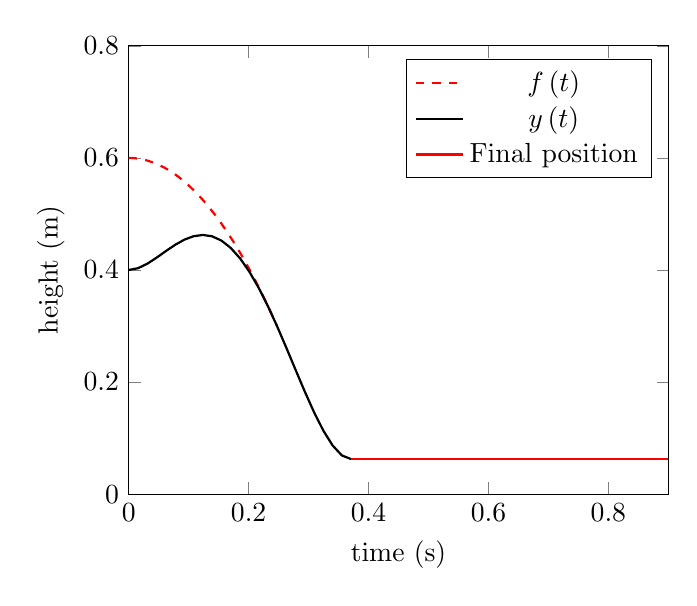
\begin{tikzpicture}
        \begin{axis}[
                xmin = 0,
                xmax = 0.9,
                ymin = 0,
                ymax = 0.8,
                xlabel = time (s),
                ylabel = height (m),
                legend pos=north east, 
                ]
            \addplot[domain = 0:0.247298674822, thick, dashed, red]{0.6-0.5*9.81*x^2};
            \addplot[domain = 0:0.37095212, thick]{160.3981*x^4-105.7772*x^3+14.7141*x^2+0.4};
            \addplot[domain = 0.37095212:0.9, red, thick]{0.0625198478831};
            \legend{$f\left(t\right)$, $y\left(t\right)$, Final position};
        \end{axis}
    \end{tikzpicture}   
	
	The origin of the height displayed is based on the pivot point of the robot arm. We know the pivot point to be 0.2 meters above the table, and since we never go negative in this graph we know:
	\begin{equation}
	y_{\textrm{min}} > 0.2
	\end{equation}
	So we stop the egg fast enough to clear the table the arm is sitting on, as 0.2 meters is greater than the minimum 0.1 meters given by the problem.

	Now we just need to convert this $y\left(t\right)$ function to polar colrdinate to find where our motor should go to. This can be done with:
	\begin{equation}
	r = \sqrt{0.25+y\left(t\right)^2}
	\end{equation}
	\begin{equation}
	\theta = \arctan(\frac{y\left(t\right)}{0.5})
	\end{equation}
	We can then add in our function of$y\left(t\right)$ and get the functions for the parameters of the acrtuators. $r$ tells us the length of the linear actuator in the arm, and $\theta$ tells us the angle of the actuator at the base of the arm. 
	\begin{equation}
	r = \sqrt{0.25+\left( 160.4 \cdot t^4 - 105.78 \cdot t^3 + 14.71 \cdot t^2 + 0.4\right)^2}
	\end{equation}
	\begin{equation}
	\theta = \arctan(\frac{160.4 \cdot t^4 - 105.78 \cdot t^3 + 14.71 \cdot t^2 + 0.4}{0.5})
	\end{equation}

	\section*{Discussion of Results}

	% needs data of actuators
	
\end{document}
